\documentclass{journal}[IEEEtran, twocolumn]             % No modificar

% PASO 1. Reemplace "Práctica 1" por el número de la práctica que corresponda
\newcommand{\dochead}{Práctica 3}     

% PASO 2. Reemplace "TÍTULO PRÁCTICA" por el título de la práctica que corresponda.
\newcommand{\docsubhead}{De RF a EC (GNURadio)}  

% PASO 3. Reemplace "B1A - 02" por el grupo de la asignatura y el número de su grupo de laboratorio
\newcommand{\teamname}{C1}     

% PASO 4. OPCIONAL: Reemplace "\docsubhead \docsubhead" por el título del documento en caso de requerirse.
\newcommand{\titulo}{\dochead: \docsubhead}      

% PASO 5. Reemplace "31 de diciembre de 2030" por la fecha de su documento
\newcommand{\fecha}{12 de octubre de 2024}      

% To load packages
\usepackage[T1]{fontenc}
\usepackage[utf8]{inputenc} 
\usepackage[spanish]{babel}
\usepackage[letter,left=2.0cm,top=2.0cm,right=2.0cm,bottom=4.0cm]{geometry}
\usepackage{amsmath}
\usepackage{amsfonts}
\usepackage{fancyhdr}
\usepackage{fancyvrb}
\usepackage{listings}
\usepackage{array}
\usepackage{graphicx,color,enumerate}	
\usepackage{multirow} 
\usepackage{multicol}
\usepackage{authblk}
\usepackage{charter}    % Font typeface
\usepackage{titling}
\usepackage{url}
\usepackage{hyperref}
\usepackage{xcolor}
\usepackage{booktabs}

\definecolor{uisgreen}{RGB}{125,194,3}
\definecolor{gray97}{gray}{.97}
\definecolor{gray75}{gray}{.75}
\definecolor{gray45}{gray}{.45}

\setlength{\droptitle}{-1.8cm}
\pagestyle{fancy}

%%% Header definition
\headheight=60pt 						% header height 
\renewcommand{\headrulewidth}{4pt}
\let\oldheadrule\headrule% Copy \headrule into \oldheadrule
\renewcommand{\headrule}{\color{uisgreen}\oldheadrule}

\fancyhead[L]							% left header 
{	\begin{minipage}{2.5cm}
		
\includegraphics[scale=0.3]{./figs/uislogohoriz.png} 
	\end{minipage}	
	\begin{minipage}{5cm}
	    \color{uisgreen}
	    \footnotesize {\textsf{Universidad Industrial de Santander\\ 
				Escuela de Ingenierías Eléctrica, \\
				Electrónica y de Telecomunicaciones	}}	
	\end{minipage}
}
\fancyhead[R] { 							%la "C" indica al centro
	\begin{minipage}{8cm}
	    \color{uisgreen}
	    \begin{flushright}
    	    \small{\textsf{Laboratorio de COMUNICACIONES I (27139)}} \\
            \normalsize{\textsf{\dochead: \textbf{\docsubhead}}} \\
    	    \small{\textsf{Grupo: \textbf{\teamname}}}
	    \end{flushright}
    \end{minipage}
    \begin{minipage}{1.2cm}
		
\includegraphics[width=1.0\textwidth]{./figs/logoE3T.png} 
	\end{minipage}	
}
%%% End header definition

\lstset{ frame=Ltb,
     framerule=0pt,
     aboveskip=0.5cm,
     framextopmargin=3pt,
     framexbottommargin=3pt,
     framexleftmargin=0.4cm,
     framesep=0pt,
     rulesep=.4pt,
     backgroundcolor=\color{gray97},
     rulesepcolor=\color{black},
     %
     stringstyle=\ttfamily\color{red!50!brown},
     showstringspaces = false,
     basicstyle=\small\ttfamily,
     commentstyle=\color{gray45},
     keywordstyle=\color{blue}\bfseries,
     %
     numbers=left,
     numbersep=15pt,
     numberstyle=\tiny,
     numberfirstline = false,
     breaklines=true,
   }

% minimizar fragmentado de listados
\lstnewenvironment{listing}[1][]
   {\lstset{#1}\pagebreak[0]}{\pagebreak[0]}

\lstdefinestyle{consola}
   {basicstyle=\scriptsize\bf\ttfamily,
    backgroundcolor=\color{gray75},
   }

\lstdefinestyle{C}
   {language=C,}             % No modificar


\begin{document}                    % No modificar

\title{\textbf{\titulo}}            % No modificar

% PASO 6. Agregar aquí el nombre y código de los autores.  
\author{
Carlos Alberto Cetina - 2215583\\
Brayan Julian Niño Hurtado - 2172301\\
Sergio Camilo Santos - 2172315\\
\href{https://github.com/scsantosdth/CommunicationsII_2024_2_scb.git}{https://github.com/scsantosdth/CommunicationsII_2024_2_scb.git}
}

\affil{\small{Escuela de Ingenierías Eléctrica, Electrónica y de Telecomunicaciones} \\ % No modificar
\small{Universidad Industrial de Santander}} % No modificar

\date{\fecha}                       % No modificar

\maketitle                          % No modificar
\thispagestyle{fancy}          % No modificar

%---------------------------------------------------------------
% PASO 7. **..**...****INICIE SU DOCUMENTO DESDE AQUI***...**...
%%%%% A PARTIR DE AQUÍ EDITE EL DOCUMENTO PARA AGREGAR TODO EL CONTENIDO REQUERIDO PARA EL ENTREGABLE CORRESPONDIENTE
%%%%  Todo el contenido a partir de este punto es SOLAMENTE ILUSTRATIVO.
%
% Para sus imformes, BORRE TODO el contenido de aquí en adelante  EXCEPTO la última línea que contiene el comando: \end{document}


\color{black}

\begin{multicols}{2}

\begin{abstract}
    En este informe se analiza el procesamiento de señales de radiofrecuencia (RF) utilizando su conversión a envolvente compleja (EC) para facilitar la modulación y demodulación. A través de GNURadio, se emplean bloques funcionales para generar y procesar señales de RF, mostrando su aplicación en sistemas de comunicación digital.
    
\end{abstract}

\section{Introducción}
  El procesamiento de señales de radiofrecuencia (RF) puede ser complejo, pero el uso de la envolvente compleja (EC) simplifica su análisis y detección de eventos importantes como picos de amplitud o cambios abruptos. Este informe utiliza GNURadio para convertir señales de RF a su forma en EC, mostrando las ventajas de esta técnica en la optimización del procesamiento de señales.


\section{Metodología}

\subsection{Parte A: Comprobar el funcionamiento del frujograma}
Se verificó el correcto funcionamiento del flujograma propuesto para la práctica, utilizando una señal OOK (On-Off Keying) tanto en su versión de radiofrecuencia (RF) como en su representación de envolvente compleja (EC) en banda base. Se hizo el analisis en el dominio del tiempo y frecuencia, comparando las señales moduladas RF y EC. Ademas, se repitieron las observaciones variando la frecuencia de la portadora, para análisis más detallado de cómo las señales RF y EC se comportan bajo diferentes condiciones. [1]


\subsection{Parte B: Comprender los bloques 'e\_RF\_VCO\_ff' y 'e\_EC\_VCO\_fc'}
Para comprender los bloques 'e\_RF\_VCO\_ff' y 'e\_EC\_VCO\_fc', se comenzó abriendo cada uno en el entorno de GNURadio y seleccionando la opción "Open in Editor" para examinar su código Python. Se modificaron los comentarios de ayuda (help) en inglés para ofrecer una explicación más detallada sobre sus parametros, entradas, salidas y operación.

\subsection{Parte C: Modulación BPSK versión RF y EC}

Para implementar la modulación BPSK en versiones RF y EC, se adaptó el flujograma inicial, activando bloques desactivados y estableciendo las interconexiones necesarias para implementar la modulación BPSK en versiones RF y EC. Y se realizaron pruebas similares a las del punto 1, aplicadas a la modulación BPSK.



\subsection{Parte E: Preguntas de control}
Preguntas de auto control sobre el flujograma randombinayrectsignal.grc
    
\section{Resultados}
\subsection{Parte A: Comprobar el funcionamiento del frujograma}


En el dominio del tiempo (Figura 1), se observó que la señal RF modulada (señal roja) sigue un comportamiento On-Off Keying (OOK), la portadora sinusoidal aparece solo cuando la señal moduladora (señal azul) es "1" y desaparece cuando es "0". Al aumentar la frecuencia de la portadora, se observó el incremento el número de ciclos de la señal sinusoidal cuando está activa.[2]

    \begin{center}
    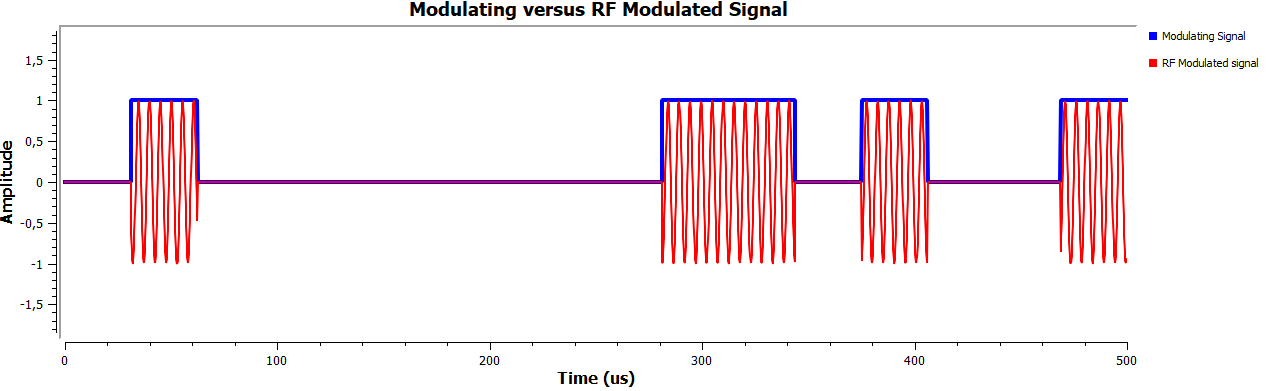
\includegraphics[width=0.45\textwidth]{figs/F1.png}
    \caption{Figura 1: Gráfica en tiempo RF modulada}
    \label{fig:1}
    \end{center}

Además, en la representación de envolvente compleja (EC) (figura 2), la componente "I" sigue los mismos patrones binarios de la señal moduladora, mientras que la componente "Q" se mantiene siempre en cero, ya que no hay información en cuadratura en la modulación OOK. 

    \begin{center}
    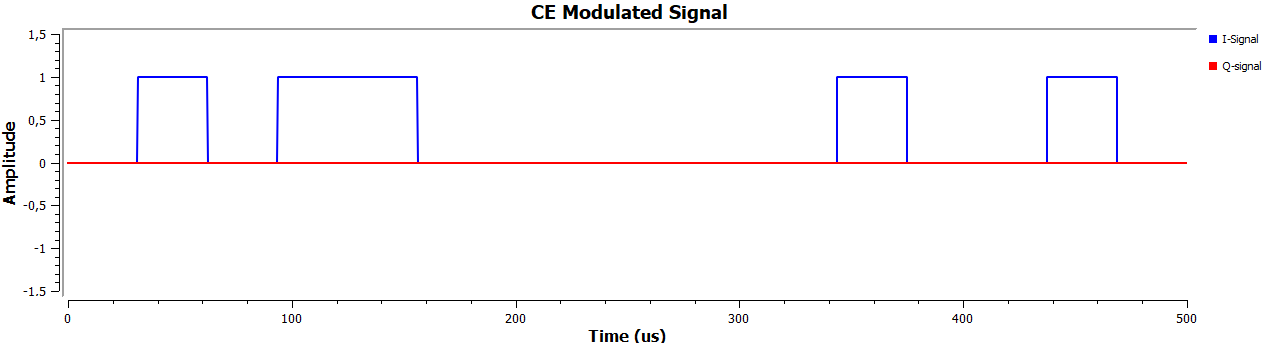
\includegraphics[width=0.45\textwidth]{figs/F2.png}
    \caption{Figura 2: Gráfica en tiempo EC modulada}
    \label{fig:2}
    \end{center}

En el dominio de la frecuencia, al modular la señal de control de amplitud (EC) con una portadora sinusoidal, se observó que la PSD de la señal modulada se desplazó hacia las frecuencias de la portadora. Este desplazamiento ocurrió debido a que la modulación OOK desplazó el contenido espectral de la señal de banda base hacia dos nuevas bandas, una centrada en la frecuencia positiva de la portadora y otra simétricamente en la frecuencia negativa. Como resultado, la PSD de la señal modulada presentó dos picos, uno en la frecuencia positiva y otro en la negativa de la portadora, replicando así la PSD de la señal EC en ambas bandas.

     \begin{center}
        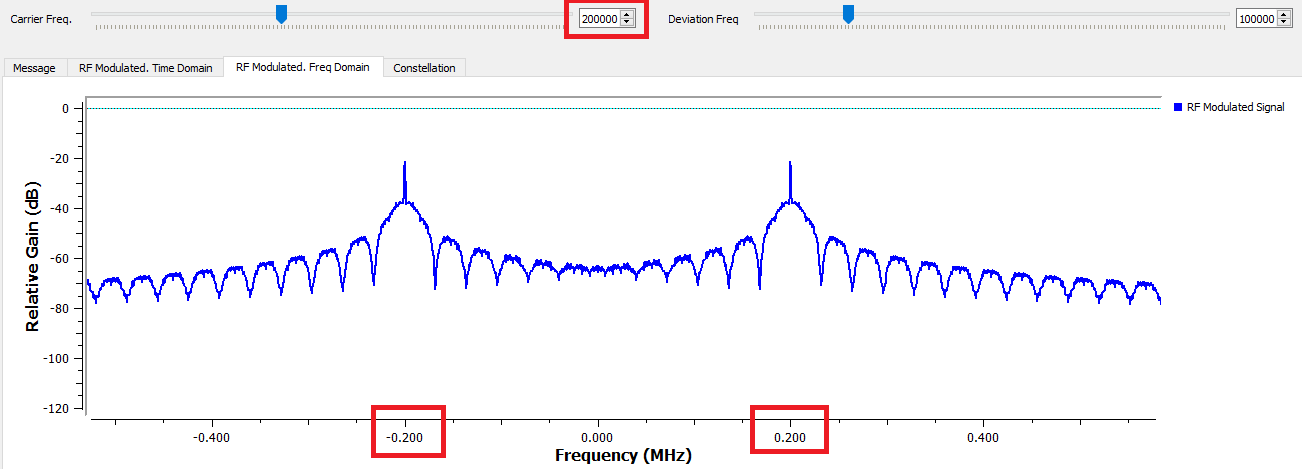
\includegraphics[width=0.45\textwidth]{figs/F3.png}
        \caption{Figura 3: PSD de la señal RF modulada}
        \label{fig:3}
    \end{center}

En el caso de la EC como se observó en la figura 4, que el espectro se concentra alrededor de la frecuencia cero, lo que refleja que la señal está en banda base y no está afectada por la portadora.

    \begin{center}
        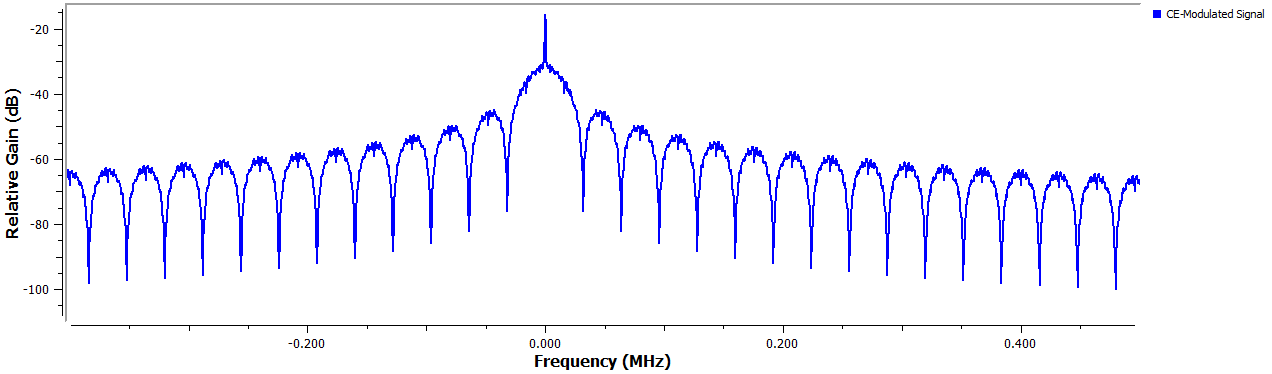
\includegraphics[width=0.45\textwidth]{figs/F4.png}
        \caption{Figura 4: PSD de la EC modulada}
        \label{fig:4}
    \end{center}
   

\subsection{Parte C: Modulación BPSK versión RF y EC}

   
\subsection{Parte B: Comprender los bloques 'e\_RF\_VCO\_ff' y 'e\_EC\_VCO\_fc'}

\begin{itemize}
 
   \item Boque: 'e\_RF\_VCO\_ff'

This block is an RF VCO that generates a sinusoidal signal with a frequency controlled by input signals. 

The parameters include \textit{fc} (Carrier Frequency), setting the oscillator's base frequency at a default of 128 kHz, and \textit{samp\_rate} which defines the number of samples per second used by the system, defaulting to 320 kHz.
  
The first input, \textit{A}, controls the output signal's amplitude, while the second input, \textit{Q}, modulates the phase. The output is a sinusoidal signal, with amplitude determined by \textit{A} and phase by \textit{Q}, and its frequency is based on \textit{fc} and the phase shift \textit{Q}.

    \item Boque: 'e\_EC\_VCO\_fc'

This block is a CE Voltage-Controlled Oscillator (VCO), or baseband VCO, and works as follows: it generates a complex sinusoidal signal based on the input signals. The block takes two input signals: 

the first input, \textit{A}, which controls the amplitude of the output signal, and the second input, \textit{Q}, which modulates the phase of the generated signal. The output is a complex-valued signal, where the real part corresponds to the in-phase component and the imaginary part to the quadrature component.
 
\end{itemize}

\subsection{Parte C: Modulación BPSK versión RF y EC}

\subsection{Parte E: Preguntas de control}

\section{Conclusiones}

\begin{itemize}
    
    \item La Conversión RF-EC es un proceso que convierte las señales en radiofrecuencia (RF) a su correspondiente Envolvente Compleja (EC). Esta transformación es fundamental en la tecnología de Radio Definida por Software (SDR), donde el software puede procesar las señales en el dominio de la EC, a diferencia de las señales RF, que físicamente viajan a frecuencias más altas. La ventaja de trabajar con EC es que permite representar y analizar señales de manera más sencilla utilizando herramientas como GNURadio.

\end{itemize}

\begin{thebibliography}{1}

\bibitem{flujgrama}
Flujograma: link

\bibitem{OOK}
Modulacion OOK: https://n9.cl/pekzh

\bibitem{comu} 
Stanford University - Lectures on Digital Communications, \textit{https://web.stanford.edu/class/ee179/lectures/notes14.pdf}

\bibitem{libro1} 
\textit{Comunicaciones Digitales basadas en radio definida por software}, ORTEGA - REYES, UIS, 2019.

\end{thebibliography}

\end{multicols}

\end{document}
